\question Suppose we want to design a telephone network connecting all the
cities, labeled $A$ to $G$, in a neighborhood. We'd like to do so at the least
cost.

\begin{center}
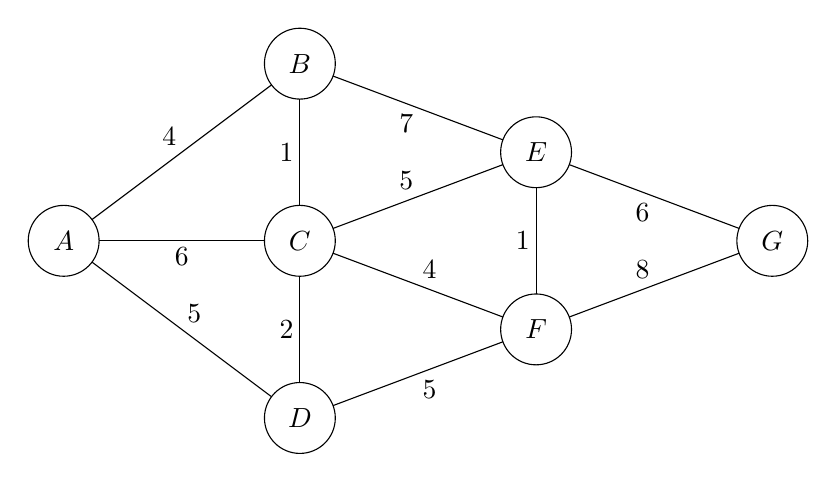
\begin{tikzpicture}[scale=0.15]
\tikzstyle{every node}+=[inner sep=0pt]
\draw (30,-15) circle (3);
\draw (30,-15) node {$B$};
\draw (10,-30) circle (3);
\draw (10,-30) node {$A$};
\draw (30,-30) circle (3);
\draw (30,-30) node {$C$};
\draw (30,-45) circle (3);
\draw (30,-45) node {$D$};
\draw (50,-37.5) circle (3);
\draw (50,-37.5) node {$F$};
\draw (50,-22.5) circle (3);
\draw (50,-22.5) node {$E$};
\draw (70,-30) circle (3);
\draw (70,-30) node {$G$};
\draw (27.6,-16.8) -- (12.4,-28.2);
\draw (18.94,-22) node [above] {$4$};
\draw (30,-18) -- (30,-27);
\draw (29.5,-22.5) node [left] {$1$};
\draw (13,-30) -- (27,-30);
\draw (20,-30.5) node [below] {$6$};
\draw (27.6,-43.2) -- (12.4,-31.8);
\draw (21.06,-37) node [above] {$5$};
\draw (30,-33) -- (30,-42);
\draw (29.5,-37.5) node [left] {$2$};
\draw (32.81,-43.95) -- (47.19,-38.55);
\draw (40.99,-41.77) node [below] {$5$};
\draw (47.19,-36.45) -- (32.81,-31.05);
\draw (40.99,-33.23) node [above] {$4$};
\draw (52.81,-23.55) -- (67.19,-28.95);
\draw (59.01,-26.77) node [below] {$6$};
\draw (67.19,-31.05) -- (52.81,-36.45);
\draw (59.01,-33.23) node [above] {$8$};
\draw (47.19,-23.55) -- (32.81,-28.95);
\draw (39.01,-25.73) node [above] {$5$};
\draw (50,-25.5) -- (50,-34.5);
\draw (49.5,-30) node [left] {$1$};
\draw (32.81,-16.05) -- (47.19,-21.45);
\draw (39.01,-19.27) node [below] {$7$};
\end{tikzpicture}
\end{center}

\begin{parts}
\part In a graph with $N$ vertices and $M$ edges, how many edges form a minimum
spanning tree?
\begin{solution}[0.5in]
$N - 1$, or 6 edges in the above graph.
\end{solution}

\part Will the new graph contain any cycles? Describe its structure.
\begin{solution}[1in]
The resulting graph is a tree which implies that it contains no cycles. If the
tree reaches every node in the graph, then it is a \define{spanning tree}.
A graph may have many spanning trees, but we are particularly interested in
\define{minimum spanning trees}, or spanning trees that minimize the total
weight of the tree.
\end{solution}

\part One algorithm to find a minimum spanning tree is Kruskal's algorithm.
\begin{enumerate}
\item Sort all the edges by increasing order of their weight.
\item Pick the smallest edge and check if it forms a cycle with the spanning
tree so far. If it doesn't form a cycle, add this edge to the spanning tree.
\item Repeat the previous step until there are $|V| - 1$ edges in the spanning
tree, where $|V|$ is the number of vertices in the graph.
\end{enumerate}

Run Kruskal's Algorithm to find a minimum spanning tree.

\begin{solution}
\begin{center}
\begin{tikzpicture}[scale=0.15]
\tikzstyle{every node}+=[inner sep=0pt]
\draw (30,-15) circle (3);
\draw (30,-15) node {$B$};
\draw (10,-30) circle (3);
\draw (10,-30) node {$A$};
\draw (30,-30) circle (3);
\draw (30,-30) node {$C$};
\draw (30,-45) circle (3);
\draw (30,-45) node {$D$};
\draw (50,-37.5) circle (3);
\draw (50,-37.5) node {$F$};
\draw (50,-22.5) circle (3);
\draw (50,-22.5) node {$E$};
\draw (70,-30) circle (3);
\draw (70,-30) node {$G$};
\draw (27.6,-16.8) -- (12.4,-28.2);
\draw (18.94,-22) node [above] {$4$};
\draw (30,-18) -- (30,-27);
\draw (29.5,-22.5) node [left] {$1$};
\draw (30,-33) -- (30,-42);
\draw (29.5,-37.5) node [left] {$2$};
\draw (47.19,-36.45) -- (32.81,-31.05);
\draw (40.99,-33.23) node [above] {$4$};
\draw (52.81,-23.55) -- (67.19,-28.95);
\draw (59.01,-26.77) node [below] {$6$};
\draw (50,-25.5) -- (50,-34.5);
\draw (49.5,-30) node [left] {$1$};
\end{tikzpicture}
\end{center}

\textbf{Meta}: Draw only the nodes and add the edges that are part of the MST
as you walk through the problem. Labeling all the edges would take a long time,
and erasing is confusing and complicated.
\end{solution}
\end{parts}
